\documentclass[a4paper, 12pt]{article}

%%% SST LAB PROTOCOLL PREAMBLE
%%% 2019
%%%%%%%%%%%%%%%%%%%%%%%%%%%%%%%


%%% PACKAGES
%%%%%%%%%%%%%%%%%%%%%%%%%%%

\usepackage[ngerman]{babel}

\usepackage[utf8]{inputenc}
\usepackage{amsmath}
\usepackage{pgfplots}
\usepackage{tikz}
\usepackage[many]{tcolorbox}
\usepackage{graphicx}
\graphicspath{ {./graphics/} }
\usepackage{pdfpages}
\usepackage{dashrule}
\usepackage{float}
\usepackage{siunitx}
\usepackage{booktabs}
\usepackage[version=4]{mhchem}

%%% DOCUMENT GEOMETRY
%%%%%%%%%%%%%%%%%%%%%%%%%%%

\usepackage{geometry}
\geometry{
 a4paper,
 total={0.6180339887498948\paperwidth,0.6180339887498948\paperheight},
 top = 0.1458980337503154\paperheight,
 bottom = 0.1458980337503154\paperheight
 }
\setlength{\jot}{0.013155617496424828\paperheight}
\linespread{1.1458980337503154}

\setlength{\parskip}{0.013155617496424828\paperheight} % paragraph spacing


%%% COLORS
%%%%%%%%%%%%%%%%%%%%%%%%%%%

\definecolor{red1}{HTML}{f38181}
\definecolor{yellow1}{HTML}{fce38a}
\definecolor{green1}{HTML}{95e1d3}
\definecolor{blue1}{HTML}{66bfbf}
\definecolor{hsblue}{HTML}{00b1db}
\definecolor{hsgrey}{HTML}{afafaf}

%%% CONSTANTS
%%%%%%%%%%%%%%%%%%%%%%%%%%%
\newlength{\smallvert}
\setlength{\smallvert}{0.0131556\paperheight}


%%% COMMANDS
%%%%%%%%%%%%%%%%%%%%%%%%%%%

% differential d
\newcommand*\dif{\mathop{}\!\mathrm{d}}

% horizontal line
\newcommand{\holine}[1]{
  	\begin{center}
	  	\noindent{\color{hsgrey}\hdashrule[0ex]{#1}{1pt}{3mm}}\\%[0.0131556\paperheight]
  	\end{center}
}

% mini section
\newcommand{\minisec}[1]{ \noindent\underline{\textit {#1} } \\}

% quick function plot
\newcommand{\plotfun}[3]{
  \vspace{0.021286\paperheight}
  \begin{center}
    \begin{tikzpicture}
      \begin{axis}[
        axis x line=center,
        axis y line=center,
        ]
        \addplot[draw=red1][domain=#2:#3]{#1};
      \end{axis}
    \end{tikzpicture}
  \end{center}
}

% box for notes
\newcommand{\notebox}[1]{

\tcbset{colback=white,colframe=red1!100!black,title=Note!,width=0.618\paperwidth,arc=0pt}

 \begin{center}
  \begin{tcolorbox}[]
   #1 
  \end{tcolorbox}
 
 \end{center} 
 
}

% box for equation
\newcommand{\eqbox}[2]{
	
	\tcbset{colback=white,colframe=hsblue!100!black,title=,width=#2,arc=0pt}
	
	\begin{center}
		\begin{tcolorbox}[ams align*]
				#1
		\end{tcolorbox}
		
	\end{center} 
	
}

% END OF PREAMBLE

%%%%%%%%%%%%%%%%%%%%%%%%%%%%%%%%%%%%%

\begin{document}

% 1
%%%%%%%%%%%%%%%%%%%%%%%%%%%%%%%%%%%%%
  
\includepdf{./titlepage/titlepage1.pdf}
  \clearpage
  \setcounter{page}{1}
%%%%%%%%%%%%%%%%%%%%%%%%%%%%%%%%%%%%%

\section{Vorbereitungsaufgaben}

\subsection{Funktion des Bipolartransistors}
\subsubsection{Spannungsgrenze}

\subsubsection{Leerlaufverstärkung}

\subsubsection{G}
-Ausgangsspannungsgrenze
-Leerlaufverstärkung
-CMRR, Gleichtakt/Gegentaktverstärkung
-Eingangsruheströme
-Gleichtakteingwiderstand differenzeingwiderstand

\subsection{Vierquadrantenkennlinienfeld}
\begin{figure}[H]
  \begin{center}
    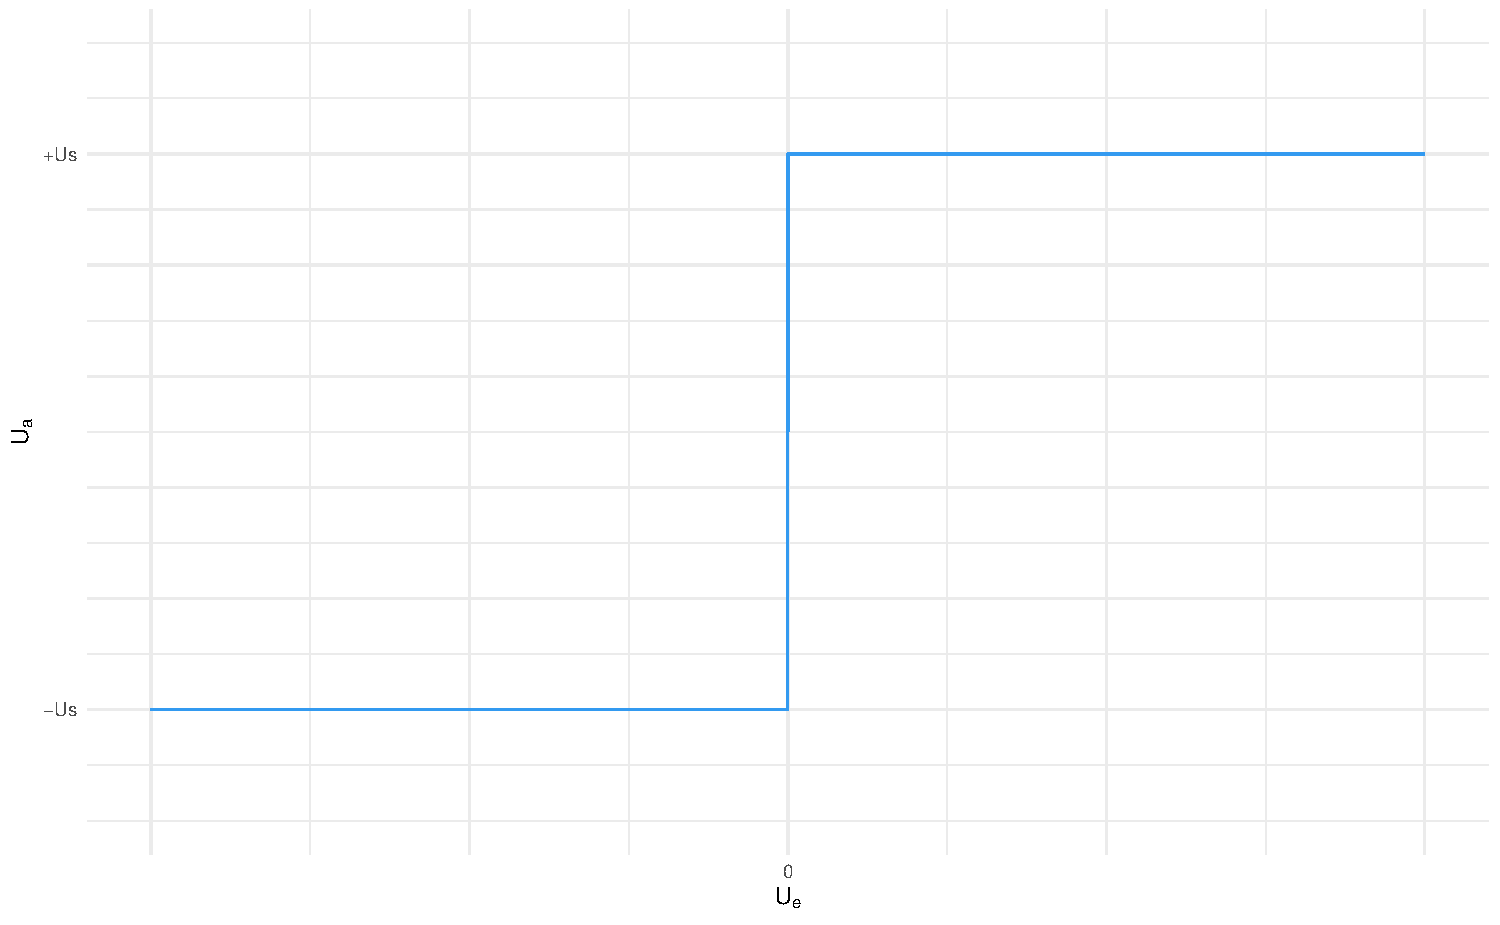
\includegraphics[width=0.618\textwidth]{1_2/opv_nofeed.pdf}
    \end{center}
    \caption{OPV-Kennlinie ohne Rückkopplung (ideal)}
 \end{figure}
\begin{figure}[H]
  \begin{center}
    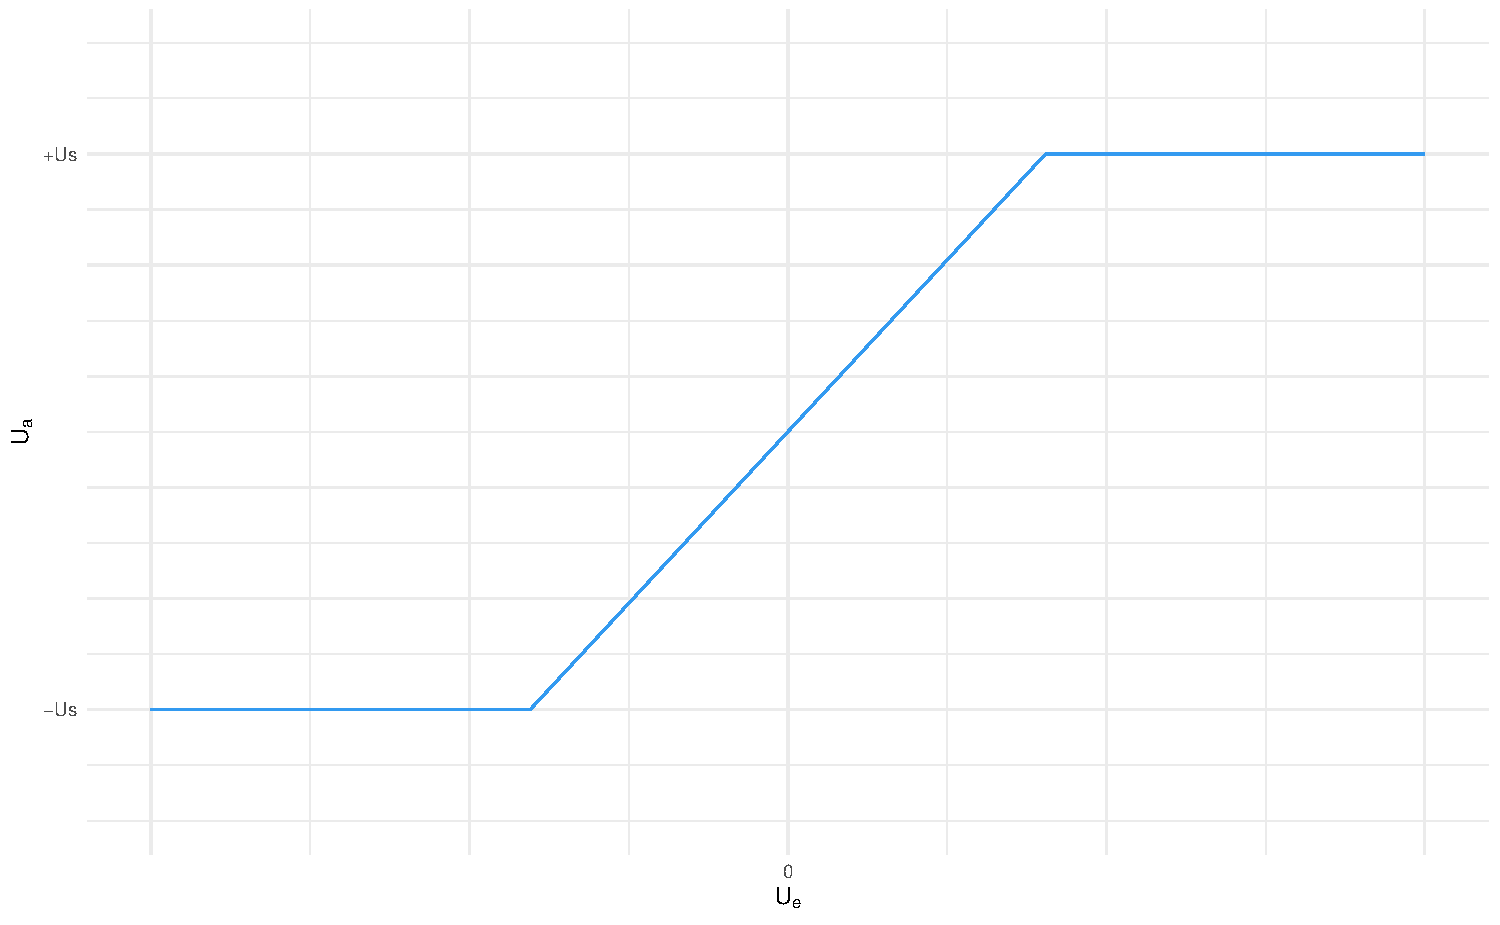
\includegraphics[width=0.618\textwidth]{1_2/opv_feed.pdf}
    \end{center}
    \caption{OPV-Kennlinie mit Rückkopplung}
 \end{figure}

Durch Rückführung eines Teils des Ausgangs- auf das Eingangssignal durch ein
Rückkopplungsnetzwerk wird der Operationsverstärker in einen linearen
Arbeitsbereich gebracht, wodurch die Verstärkung nicht mehr den Wert der der Leerlaufverstärkung (Abb. 1), sondern einen kontrollierten Verstärkungswert (Abb. 2) annimmt.


\subsection{Vierpolersatzschaltbild}
  \begin{figure}[H]
\begin{center}
    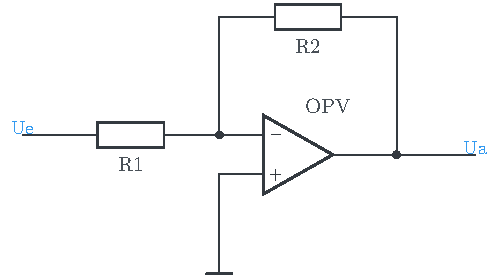
\includegraphics[width=0.618\textwidth]{circuits/inv_verst.pdf}
\end{center}
    \caption{Invertierende Verstärkerschaltung}
  \end{figure}

\begin{gather*}
  U_a = V_0(U_p-U_n)\\
  U_p = 0 \, \si{\volt}\\
  U_a = -V_0 \cdot U_n\\
  \intertext{Bestimmung von $U_n$ durch Überlagerung der Eingangs- und
    Ausgangswirkung:}
  U_n = U_n' + U_n''\\
  U_n' = U_n|_{U_a=0}\\
  = U_e \cdot \frac{R_2}{R_1 + R_2}\\
  U_n'' = U_n|_{U_e=0}\\
  = U_a \cdot \frac{R_1}{R_1 + R_2}\\
  U_a = -V_0 \cdot U_e \cdot \frac{R_2}{R_1+R_2} - V_0 \cdot U_a \cdot
  \frac{R_1}{R_1+R_2}\\
  U_a (1 + V_0 \cdot \frac{R_1}{R_1+R_2}) = -V_0 \cdot U_e \cdot \frac{R_2}{R_1+R_2}\\
  \frac{U_a}{U_e} = V = - \frac{V_0 \cdot \frac{R_2}{R_1+R_2}}{1+V_0 \cdot
    \frac{R_1}{R_1+R_2}} = - \frac{V_0}{(R_1+R_2) + V_0 \cdot R_1}\\
  V = - \frac{R_2}{\frac{R_1+R_2}{V_0} + R_1}\\
  \intertext{für $V_0 \rightarrow \infty$}
  V = -\frac{R_2}{R_1}
\end{gather*}

\subsection{Transistorgrundschaltungen}
\begin{figure}[H]
  \begin{center}
    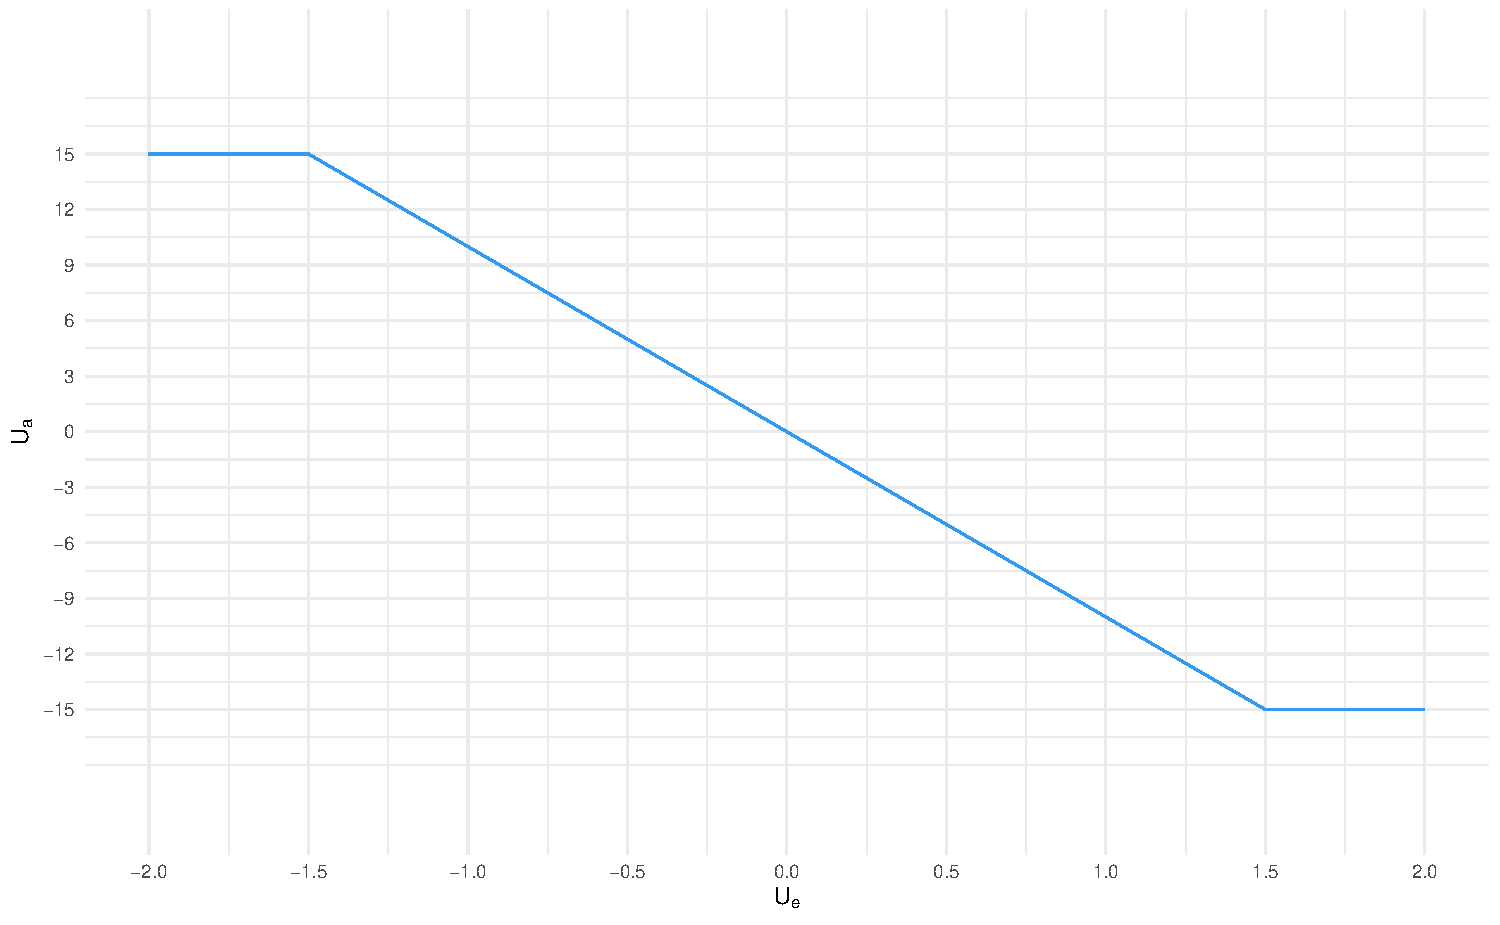
\includegraphics[width=\textwidth]{1_4/opv_inv_verst.pdf}
    \end{center}
    \caption{Kennlinie eines (idealen) OPV mit einer Verstärkung von $V_u = -10$ und einer
      Versorgungsspannung von $U_s = \pm 15 \, \si{\volt}$}
 \end{figure}


\subsection{Emitterstufe}


\subsection{Temperaturabhängigkeiten}
Temperaturänderungen stellen für den Transistor als Halbleiterbauelement eine
externe Energiezufuhr und damit eine Störung des thermodynamischen
Gleichgewichts dar. Die Ladungsträgerdichten der einzelnen Bereiche
erhöhen sich, die Weiten der Raumladungszonen verringern sich und der Transistor
wird insgesamt leitfähiger. Dadurch erhöht sich auch der
Stromverstärkungsfaktor $\beta$, was z.B. den Arbeitspunkt, der bei der
Schaltungsdimensionierung angenommen wurde, verschieben kann. Da dieser zusätzlich
fertigungsbedingt abweichen kann, strebt man einen
Arbeitspunkt an, der möglichst unabhängig von der Stromverstärkung ist. Dies
wird z.B. durch die Arbeitspunkteinstellung mit einem 4-Widerstandsnetzwerk oder
die Einstellung des Emitterstroms durch eine Stromquelle erreicht.



Bootstrapping ist eine Art der positiven Rückkopplung

\end{document}
